\section{Background \& Motivations}

\subsection{Multi-Agent Systems}
\begin{frame}{Multi-Agent Systems}
    \begin{columns}
        \begin{column}{0.45\textwidth}
            \begin{itemize}
                \item The model chosen by \emph{IntellIoT} for designing and implementing complex IoT systems is represented by \textbf{Multi-Agent Systems} (MAS)
            \end{itemize}
        \end{column}
        \begin{column}{0.55\textwidth}
            \begin{figure}
                \centering
                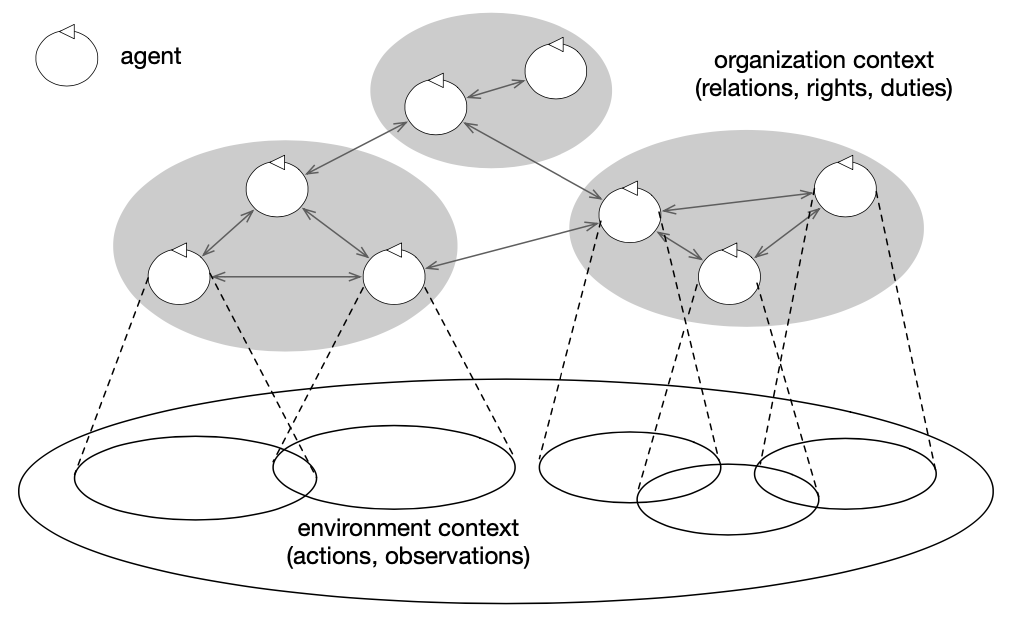
\includegraphics[width=0.8\textwidth]{images/multi-agent-systems.png}
            \end{figure}
        \end{column}
    \end{columns}

    \vspace{0.5cm}

    \begin{block}{Multi-Agent System}
        A MAS consists of multiple decision-making agents interacting in a shared environment to achieve common or conflicting goals~\cite{turing}
    \end{block}
\end{frame}

\begin{frame}{Multi-Agent Oriented Programming}
    \begin{block}{Multi-Agent Oriented Programming}
        MAOP is an approach to programming MAS that promotes the use of three first-class programming abstractions: the \textbf{agent} dimension, the \textbf{environment} dimension, and the \textbf{organization} dimension~\cite{boissier2020multi}
    \end{block}

    \begin{columns}
        \begin{column}{0.4\textwidth}
            \begin{itemize}
                \item JaCaMo is the open-source technology adopted to support the integration of tools and languages for programming the three dimensions of MAOP~\cite{boissier2020multi}
            \end{itemize}
        \end{column}
        \begin{column}{0.6\textwidth}
            \begin{figure}
                \centering
                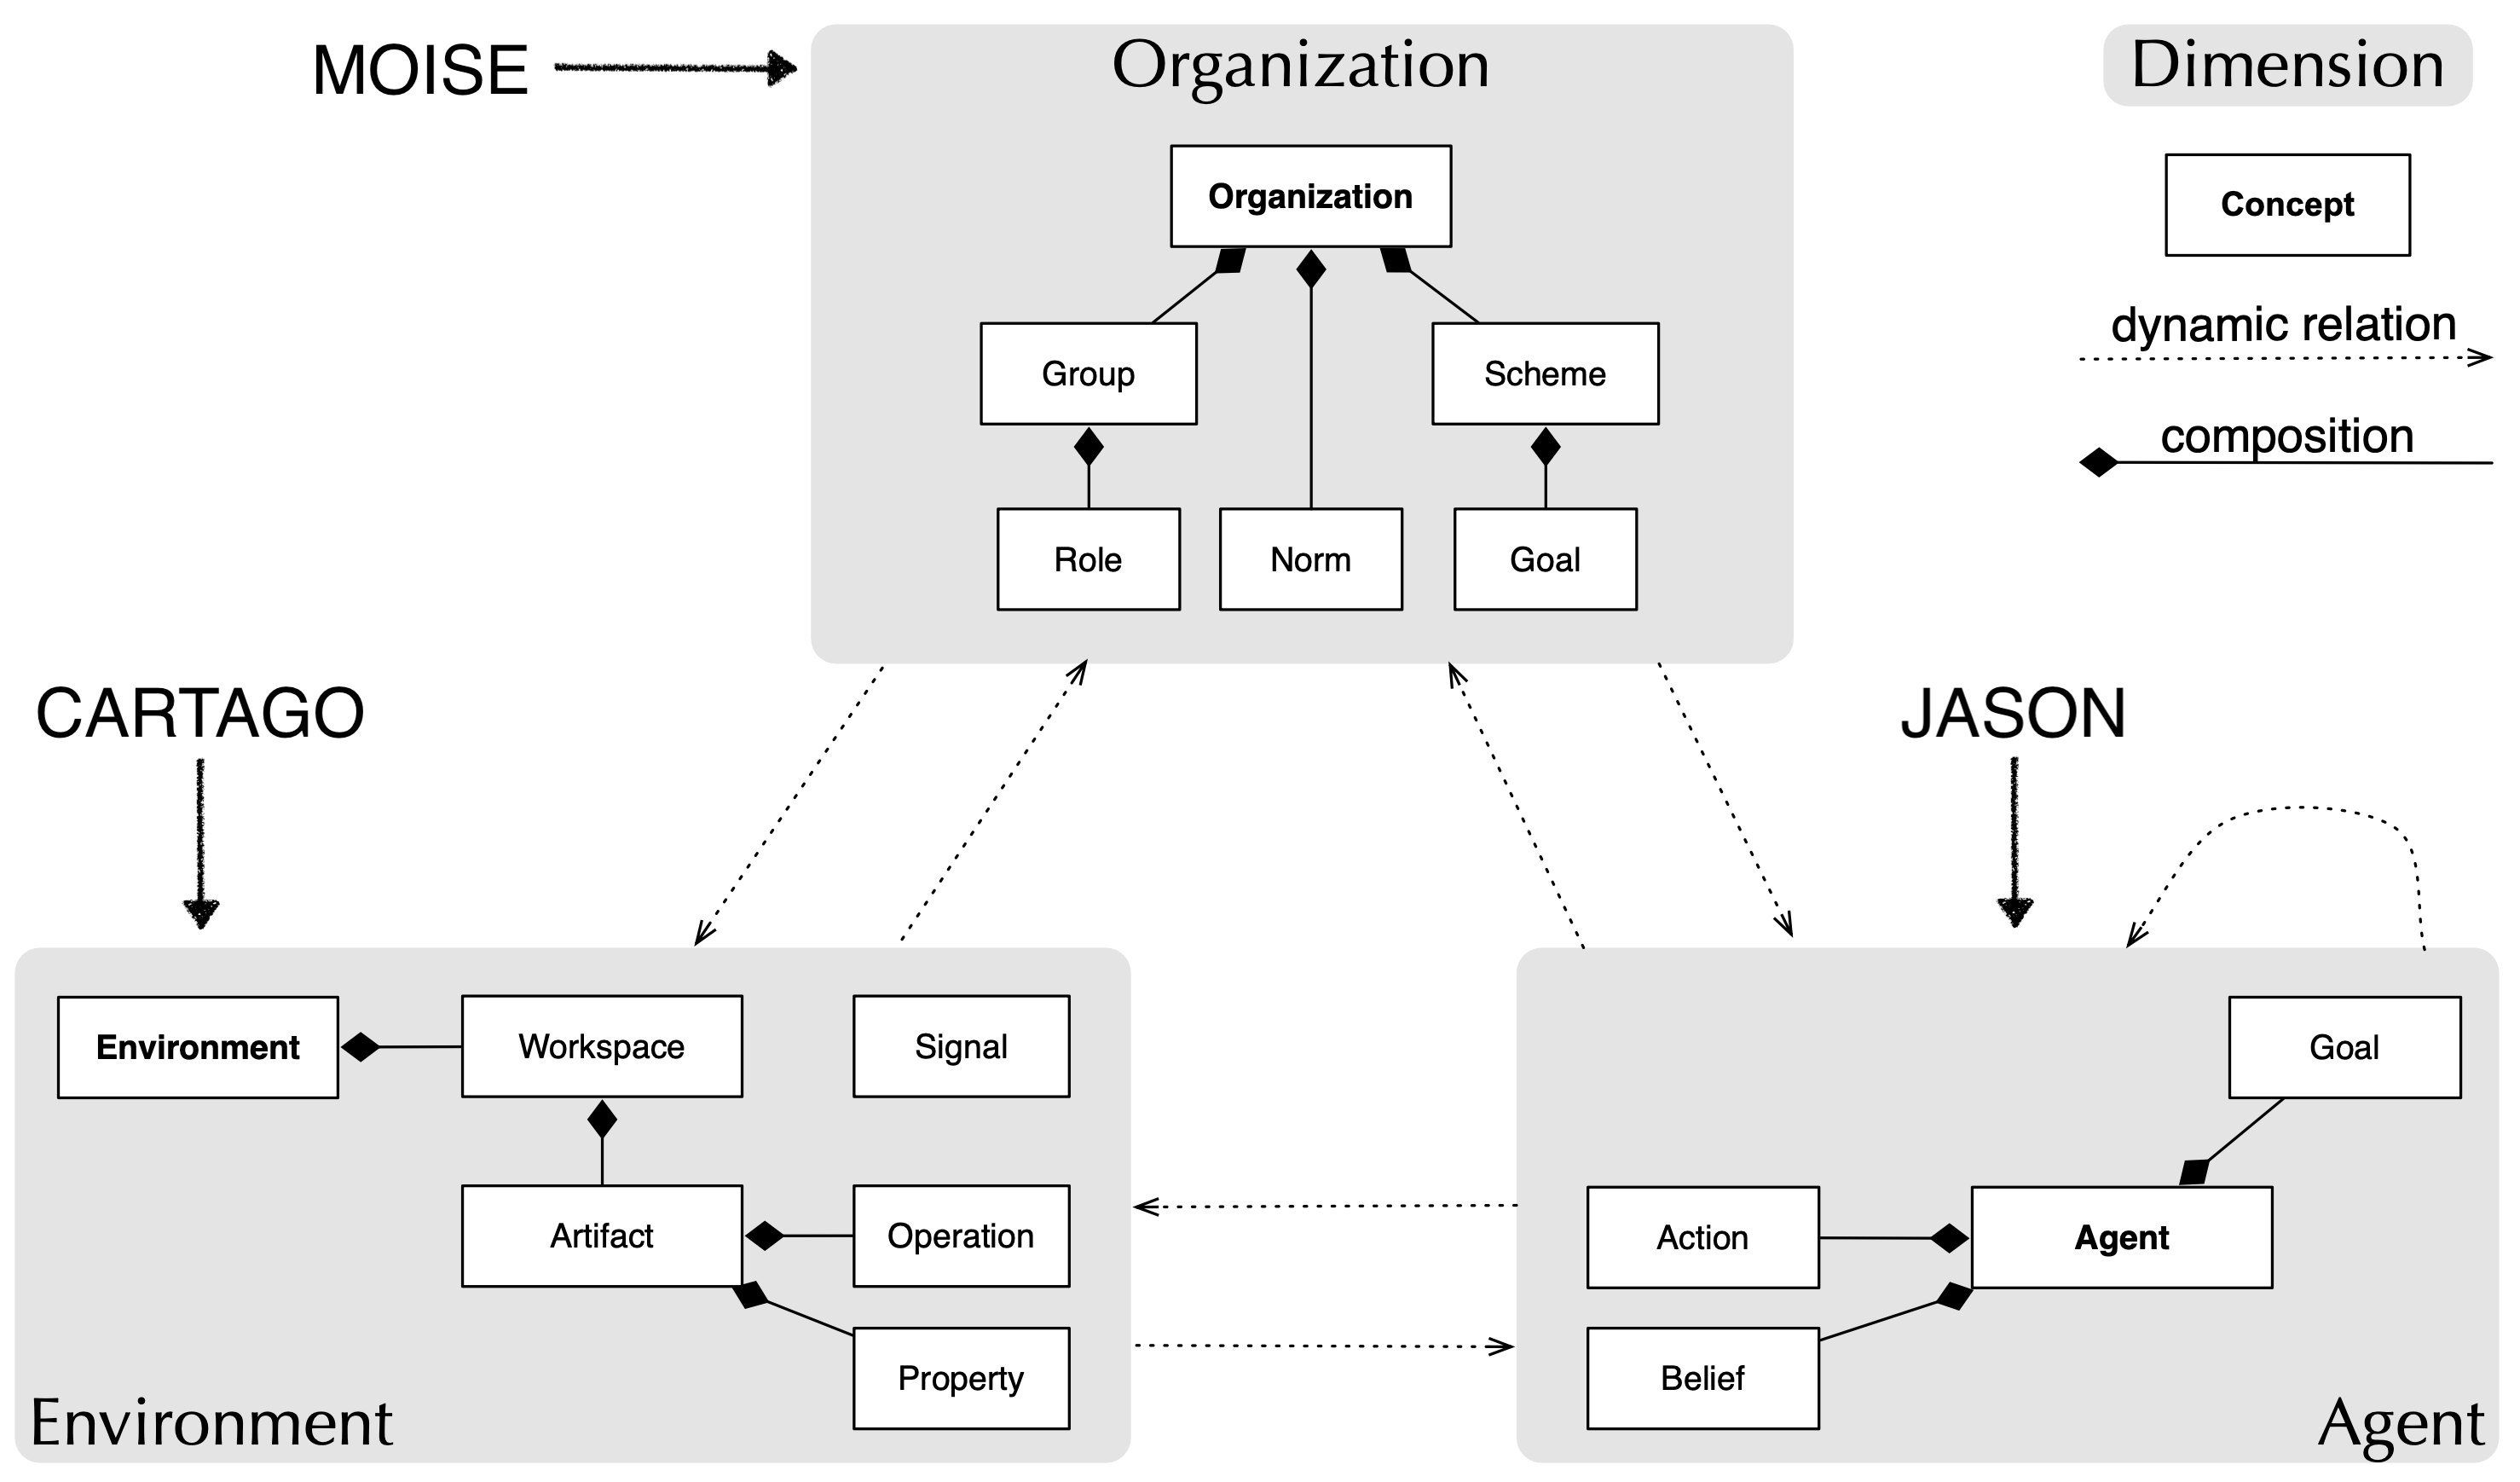
\includegraphics[width=0.9\textwidth]{images/maop.png}
            \end{figure}
        \end{column}
    \end{columns}
\end{frame}

\subsection{Domain Expert Programming}
\begin{frame}{Domain Expert Programming}
    \begin{itemize}
        \item Domain experts are the most suitable for designing solutions for domain-specific problems thanks to their \textbf{expertise}
        \vspace{0.5cm}
        \item The aim is to provide them with user-friendly tools to ground their ideas into a concrete implementation
        \vspace{0.5cm}
        \item Intuitiveness is the key point: the tools should reflect the domain experts' mental model
    \end{itemize}
\end{frame}

\subsection{Visual Programming for MAS}
\begin{frame}{Visual Programming for MAS}
    \begin{columns}
        \begin{column}{0.5\textwidth}
            \begin{itemize}
                \item A block-based visual programming language for agents already exists~\cite{burattini2022agent}\dots
                \item \dots BUT
            \end{itemize}
        \end{column}
        \begin{column}{0.5\textwidth}
            \begin{figure}
                \centering
                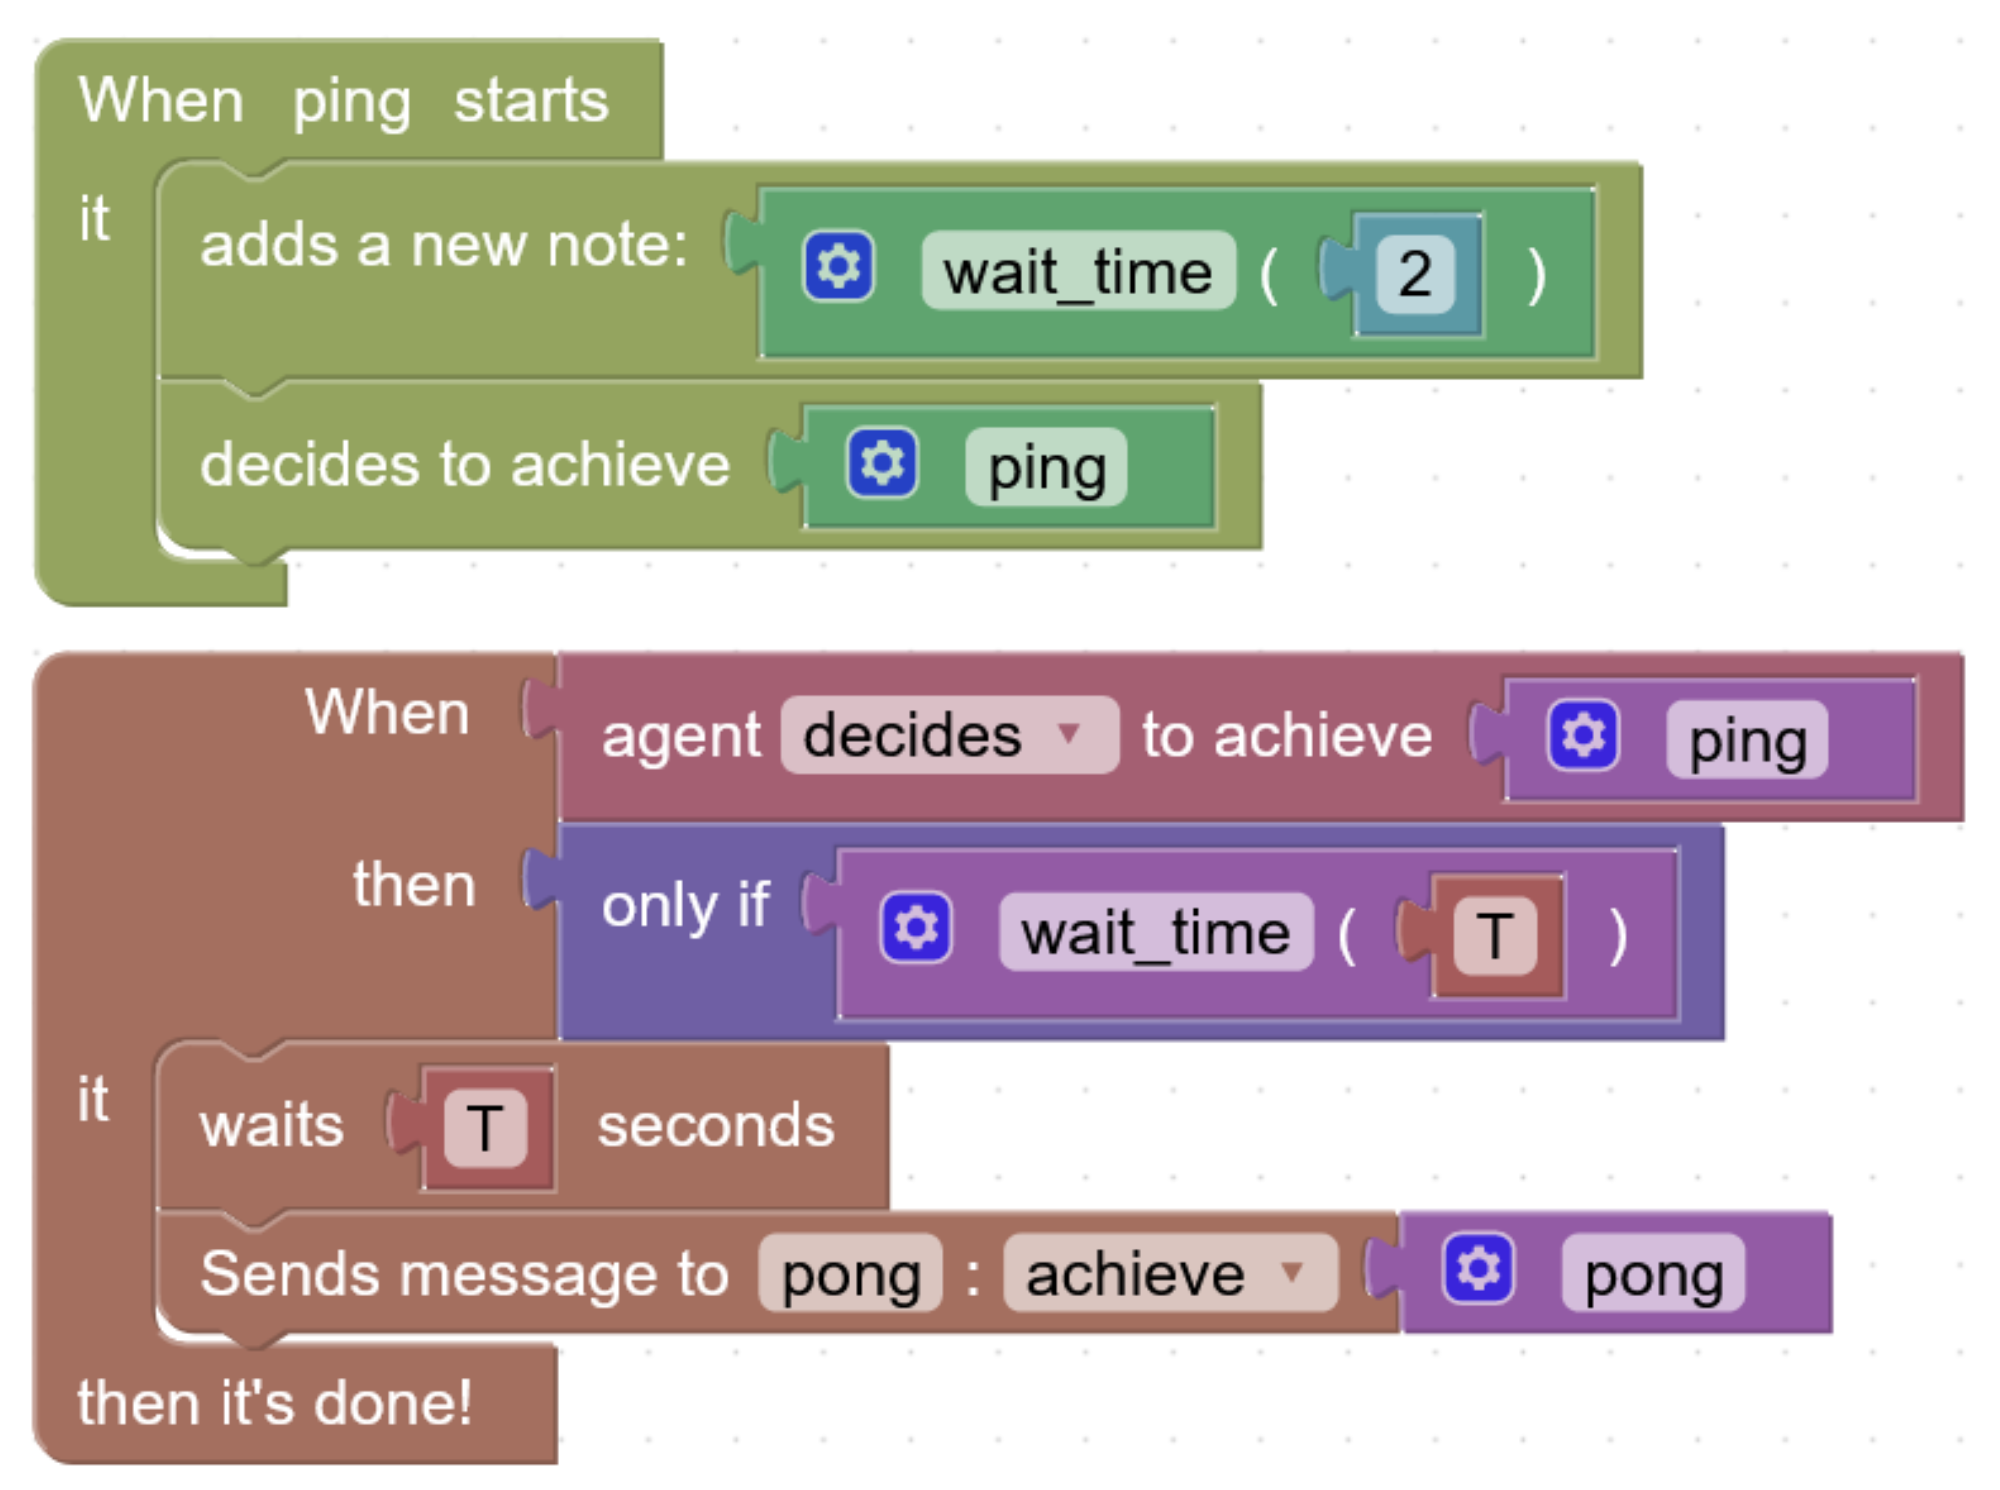
\includegraphics[width=0.9\textwidth]{images/blocks-example.png}
            \end{figure}
        \end{column}
    \end{columns}

    \begin{block}{Challenge}
        Dealing with \textbf{interaction} and \textbf{coordination} between agents in complex systems directly inside the agents makes the design of the system exponentially complex
    \end{block}
\end{frame}
